\documentclass[../main.tex]{subfiles}

\begin{document} %%%%%%%%%%%%%%%%%%%%%%%%%%%%%%%%%%%%%%%%%%%%%%%%%%%%%%%%%%%%
\section{Grafos} 
    Lista de reproducción YouTube \cite{grafos_lista_youtube}.

    \subsection{Propiedades}
    
    % Cargamos la imagen
    \begin{figure}[ht]
        \centering
        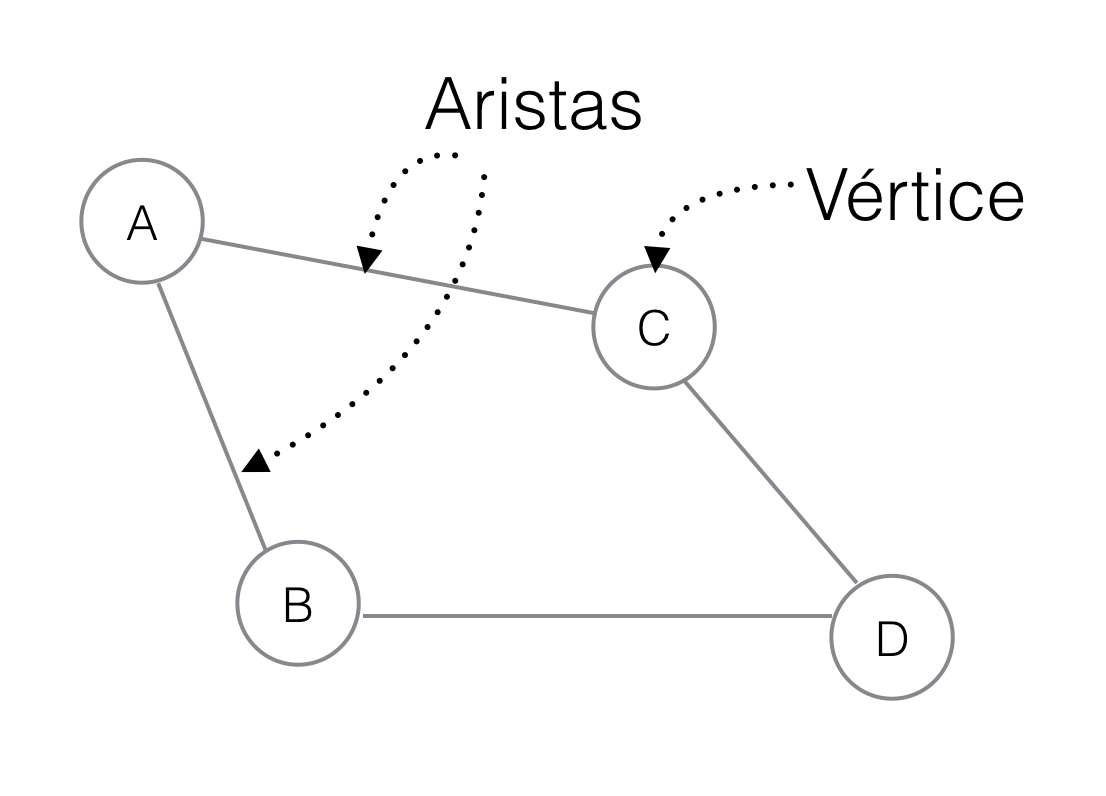
\includegraphics[width=0.5\textwidth]{images/grafos/grafo_aristas_vertices.png}
        \caption{Aristas = Edge y Vértices o Nodos = Vertex }
    \end{figure}


    \begin{enumerate}
        \item \textbf{Grafos orientados} (o dirigidos o digrafos) si las aristas (o arcos) que conectan sus vertices
        (también llamados nodos) están orientadas.
        \item \textbf{Grafos no orientados} (o no dirigidos) si las aristas que conectan sus vertices no están
        orientadas.
            % Cargamos la imagen
            \begin{figure}[ht]
                \centering
                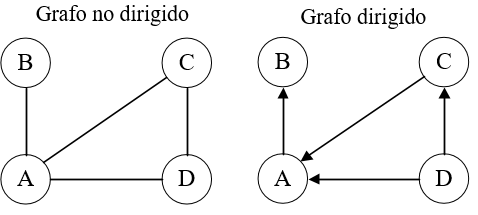
\includegraphics[width=0.5\textwidth]{images/grafos/grafos_dirigido.png}
                \caption{Grafos Dirigido y No Dirigido}      
            \end{figure}

        \item \textbf{Ciclo:} camino que conteniendo vertices distintos, excepto el primero que coincide con el ultimo.
            % Cargamos la imagen
            \begin{figure}[ht]
                \centering
                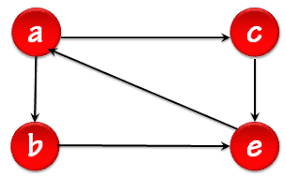
\includegraphics[width=0.3\textwidth]{images/grafos/grafo_ciclo.png}
                \caption{Grafos Ciclo: $a \rightarrow b \rightarrow e \rightarrow a$, longitud 3.}
                \label{fig:grafos_ciclo}     
            \end{figure}

        \item \textbf{Grafo no dirigido conexo:} Grafo no orientado es conexo si para todo vértice del grafo hay un camino que lo conecte con otro vertice cualquiera del grafo.
            % Cargamos la imagen
            \begin{figure}[ht]
                \centering
                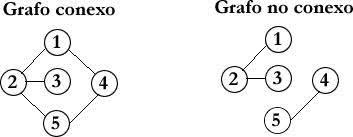
\includegraphics[width=0.5\textwidth]{images/grafos/grafo_conexo.jpeg}
                \caption{Grafos Conexo y No Conexo}
            \end{figure}
        
        \item \textbf{Grafo dirigido fuertemente conexo:} Grafo dirigido es fuertemente conexo sii entre cualquier par de vértices hay un camino que los une. Ver Figura \ref{fig:grafos_ciclo}.
        
        \item \textbf{Árbol libre:} Grafo no dirigido conexo sin ciclos.
            % Cargamos la imagen
            \begin{figure}[ht]
                \centering
                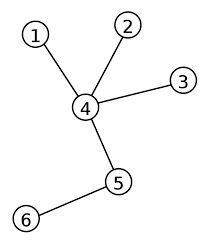
\includegraphics[width=0.3\textwidth]{images/grafos/grafo_arbol_libre.png}
                \caption{Grafos Árbol Libre}
            \end{figure}
    \end{enumerate}
    
    \newpage

    \subsection{Estructuras para implementar grafos}

        \subsubsection{Matriz de Adyacencia}
            \underline{Propiedades de la matriz de adyacencia:}
            \begin{itemize}
                \item \textbf{Grafo no dirigido:} La matriz de adyacencia es simétrica.
            \end{itemize}

            % Cargamos la imagen
            \begin{figure}[ht]
                \centering
                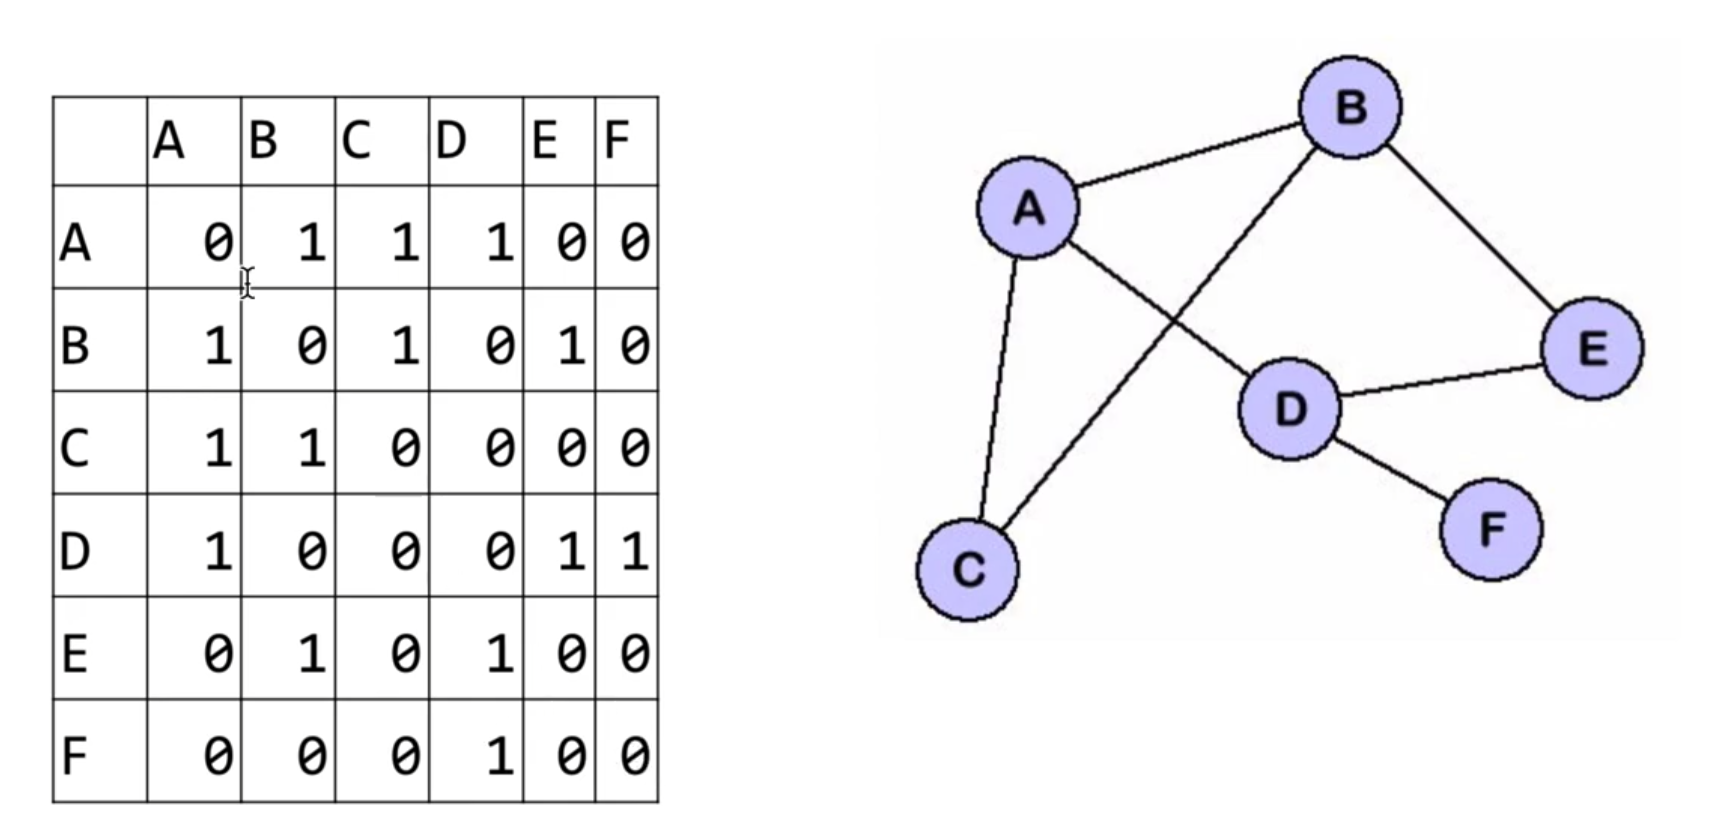
\includegraphics[width=0.8\textwidth]{images/grafos/grafo_matriz_adyacencia_1.png}
                \caption{Grafo no dirigido y no pesado Matriz de Adyacencia} 
            \end{figure}

            % Cargamos la imagen
            \begin{figure}[ht]
                \centering
                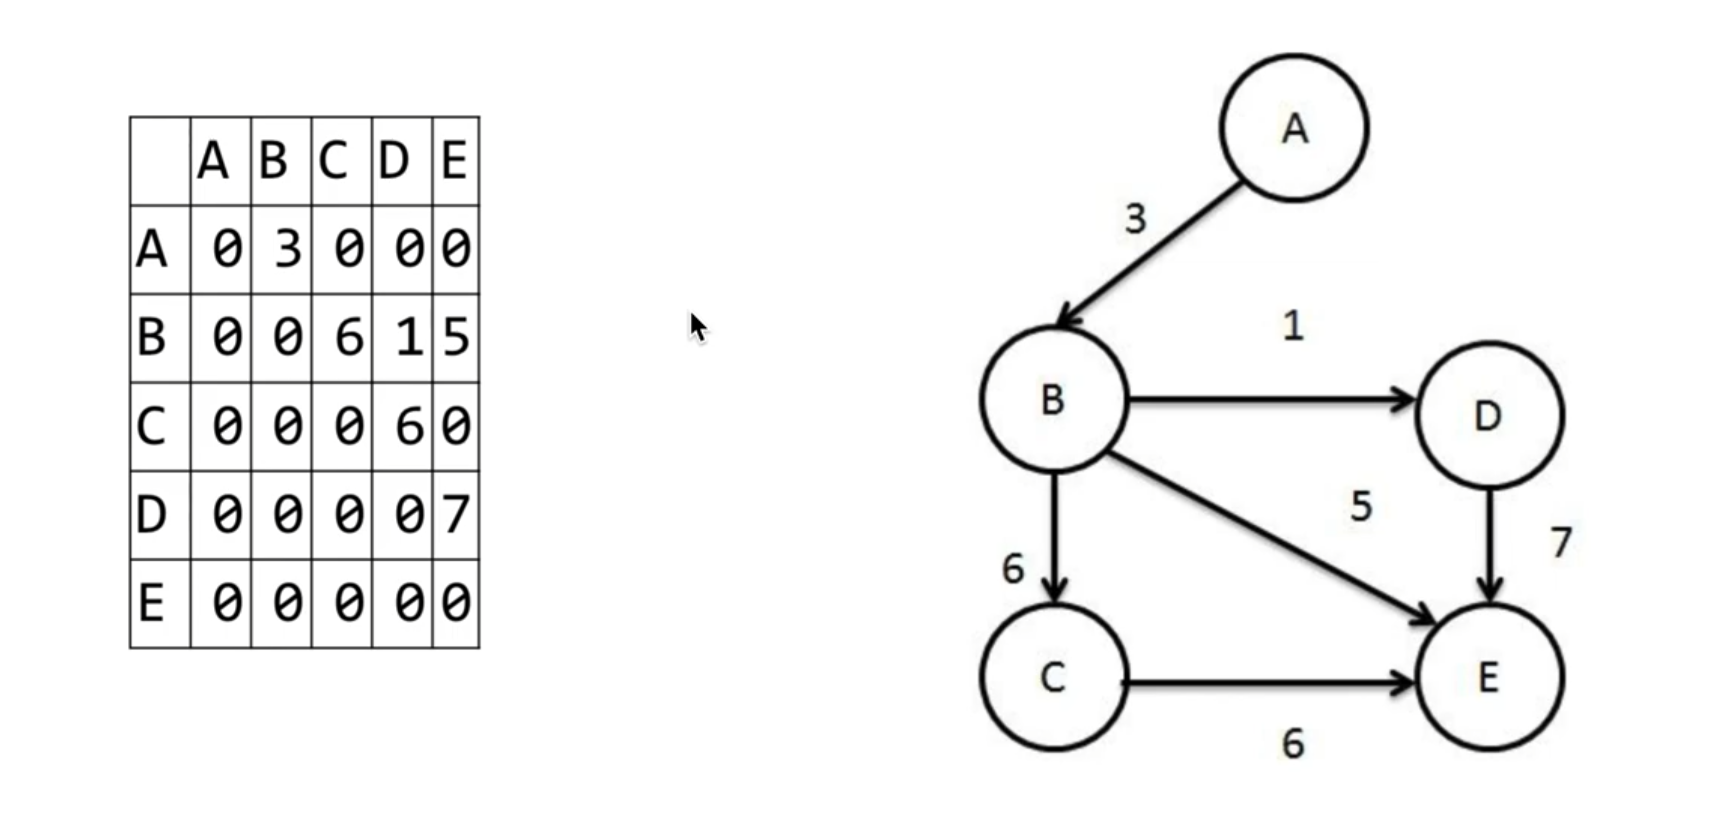
\includegraphics[width=0.8\textwidth]{images/grafos/grafo_matriz_adyacencia_2}
                \caption{Grafo dirigido y pesado Matriz de Adyacencia} 
            \end{figure}
            
            \newpage

        \subsubsection{Matriz de Incidencia}
            % Cargamos la imagen
            \begin{figure}[ht]
                \centering
                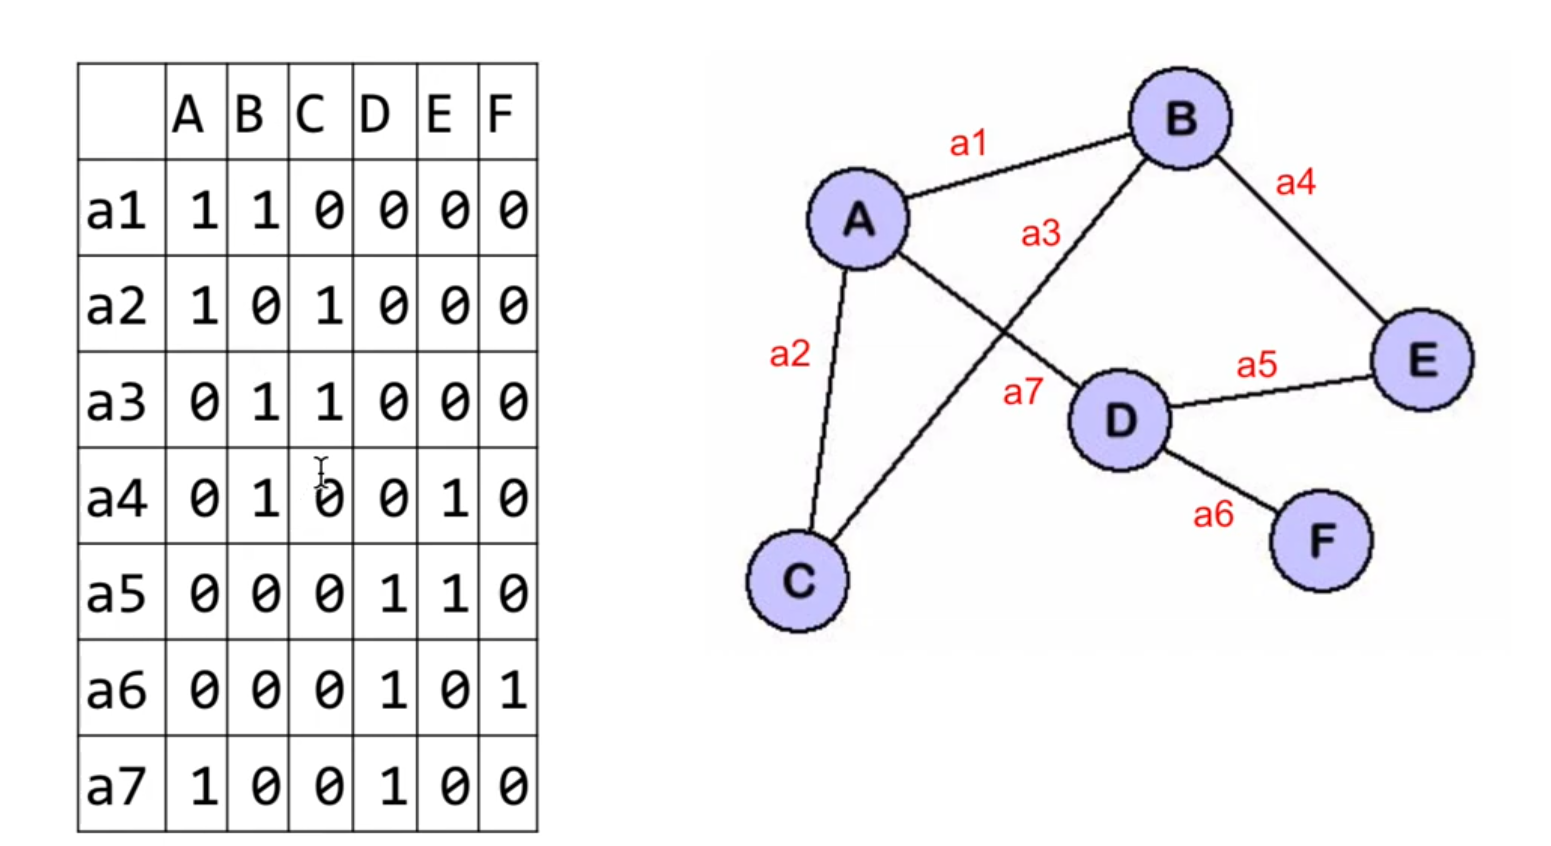
\includegraphics[width=0.8\textwidth]{images/grafos/grafo_matriz_incidencia_1.png}
                \caption{Grafo no dirigido y no pesado} 
            \end{figure}

            % Cargamos la imagen
            \begin{figure}[ht]
                \centering
                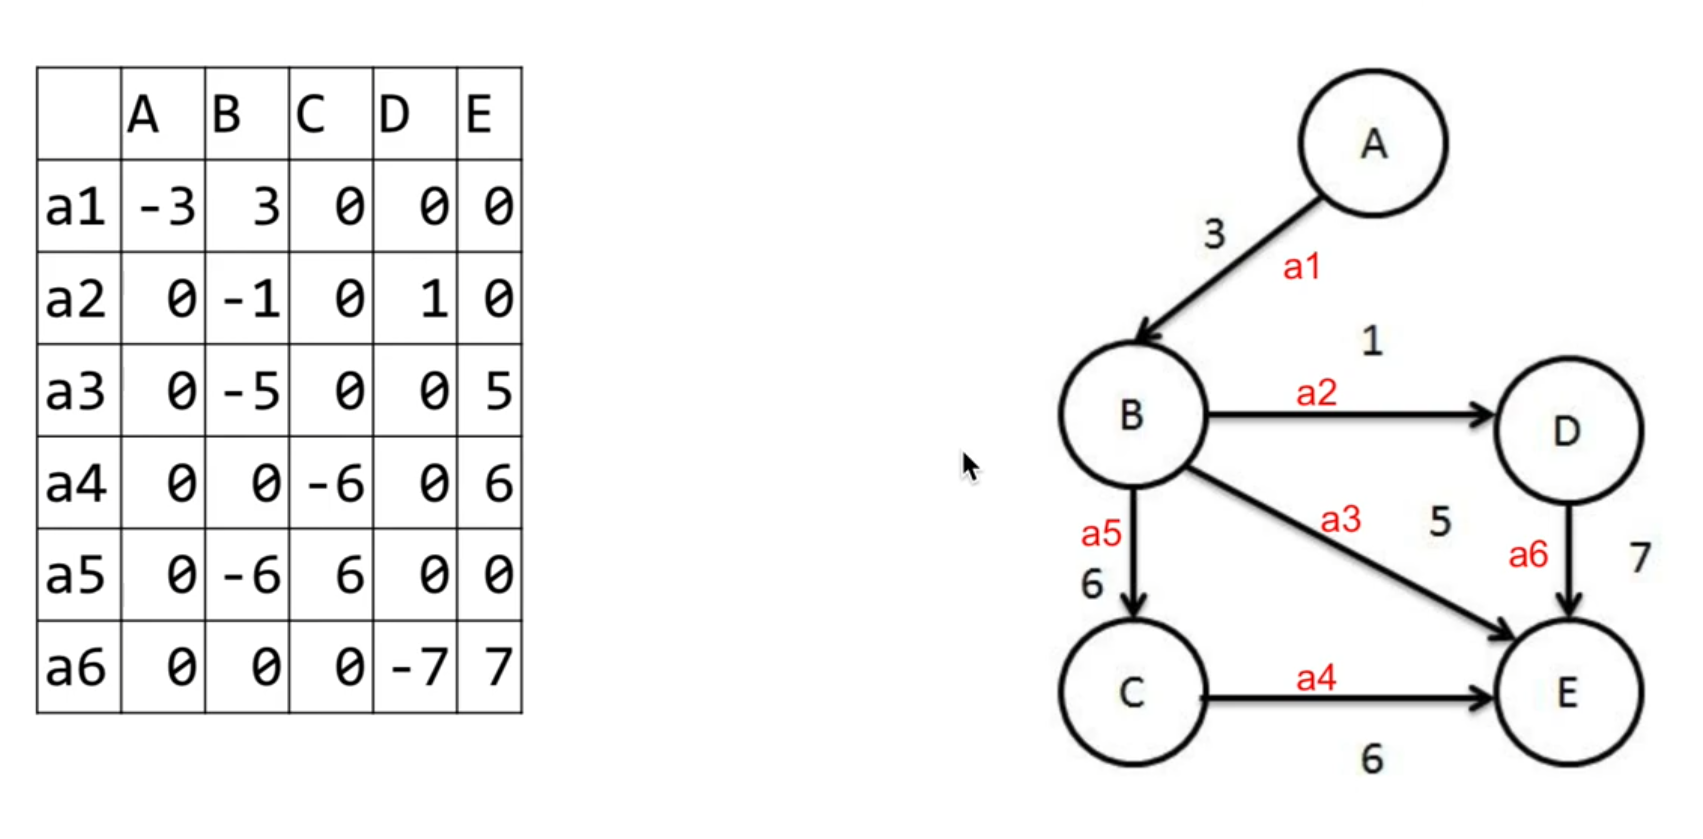
\includegraphics[width=0.8\textwidth]{images/grafos/grafo_matriz_incidencia_2.png}
                \caption{Grafo dirigido y pesado Matriz de Incidencia} 
            \end{figure}

            \newpage

            \subsubsection{Complejidad}
    
                \begin{table}[ht]
                    \centering
                    \begin{tabular}{|l|l|l|l|}
                    \hline
                        & M. Incidencia & M. Adyacencia & Lista Adyacencia\\ \hline
                        \textbf{Espacio:} & $O(V \cdot E)$ & $O(V^2)$ & $O(V + E)$\\ \hline
                        \textbf{Agregar un vértice:}  & $O(V \cdot E)$ & $O(V^2)$ & $O(1)$ o $O(V)$\\ \hline
                        \textbf{Agregar una arista:} & $O(V \cdot E)$ & $O(1)$ & $O(V)$ \\ \hline
                        \textbf{Si dos vértices son adyacentes:} & $O(E)$ & $O(1)$ & $O(V)$\\ \hline
                        \textbf{Obtener los abyacentes de un vértices:} & $O(E)$ & $O(V)$ & $O(V)$\\ \hline
                    \end{tabular}
                    \caption[short]{Coplejidad.}
                \end{table}

        \subsection{Recorridos Grafos}
            \underline{Recorridos Grafos Dirigidos}
            \begin{itemize}
                \item Anchura: BFS (Breadth First Search)
                \item Profundidad: DFS (Depth First Search)
            \end{itemize}

      
            \paragraph{BFS:} Se lo puede implementar con una cola (es mas fácil verlo de esta manera).
            \paragraph{DFS:} Se lo puede implementar con recursividad (es mas fácil verlo de esta manera) o con una pila. Cuando se trabaja con grafos No conexos se puede implementar el algoritmo para que recorra todos los nodos no visitados.\\

            \underline{Referencias:}
            \begin{itemize}
                \item Video YouTube - Recorrido DFS Recursividad FIUBA \cite{grafo_dfs_recursividad_youtube}.
                \item Video YouTube - Recorrido BFS y DFS con Pilas y Colas  \cite{grafo_bfs_dfs_youtube_1}.
                \item Video YouTube - Recorrido BFS y DFS con Pilas y Colas  \cite{grafo_bfs_dfs_youtube_2}.
                \item Página simula recorrido BFS y DFS tiene errores \cite{grafo_bfs_dfs_simulacion_1}.
                \item Página simula recorrido BFS y DFS SIN errores \cite{grafo_bfs_dfs_simulacion_2}.
            \end{itemize}


            \subsubsection{BFS: Recorrido en Anchura}
                Para grafos dirigidos y no dirigidos.\\
                
                \underline{Procedimento:}
                \begin{itemize}
                    \item Seleccionar un vértice inicial.
                    \item Marcarlo como visitado.
                    \item Encolarlo.
                    \item Mientras la \textbf{cola} (FIFO) no esté vacía :
                        \begin{itemize}
                            \item Desencolar vértice.
                            \item Mostrarlo.
                            \item Marcar como visitados.
                                \begin{itemize}
                                    \item Los vertices adyacentes no visitado.
                                \end{itemize}
                                \item Encolar.
                        \end{itemize}

                \end{itemize}

            \subsubsection{DFS: Recorrido en Profundidad}
                Para grafos dirigidos y no dirigidos.\\
                
                \underline{Procedimento:}
                \begin{itemize}
                    \item Seleccionar un vértice inicial.
                    \item Marcarlo como visitado.
                    \item Apilarlo.
                    \item Mientras la \textbf{pila} (LIFO) no esté vacía :
                        \begin{itemize}
                            \item Desapilar vértice.
                            \item Mostrarlo.
                            \item Recorrer todos los vértices adyacentes del vértice desapilado
                                \begin{itemize}
                                    \item Si el vértice adyacente no ha sido visitado, marcarlo como visitado y apilarlo.
                                    \item Si el vértice adyacente ya ha sido visitado, continúa con el siguiente vértice adyacente.
                                \end{itemize}
                        \end{itemize}
                \end{itemize}

            \subsubsection{Complejidad BFS y DFS}
                
                \begin{table}[ht]
                    \centering
                    \begin{tabular}{|l|l|l|}
                    \hline
                    & Matriz Adyacencia & Matriz Incidencia  \\ \hline
                    Anchura BFS & $O(V^2)$ & $O(V+E)$ \\ \hline
                    Profundidad DFS & $O(V^2)$ & $O(V+E)$  \\ \hline
                    \end{tabular}
                    \caption[short]{Coplejidad.}
                    \label{tab:tabla_complejidad_bfs_dfs}
                \end{table}

            \subsubsection{Aplicaciones}
                \underline{DFS: Recorrido Profundidad}
                \begin{enumerate}
                    \item \textbf{Test de Aciclidad (Ciclos):} Se recorre el grafo teniendo en cuenta los recorridos paciales. Cl coste del algorimos es el mismo que la Tabla \ref{tab:tabla_complejidad_bfs_dfs}.
                    \item  \textbf{Puntos de Articulación:} Un punto de articulación (o vértice de corte) de un grafo \textbf{no dirigido} y \textbf{conexo} es un vértice que verifica que al ser eliminado del grafo éste deja de ser conexo.
                    \item \textbf{Obtención de las componentes fuertemente conexas en un grafo dirigido:} Una componente fuertemente conexa es un subgrafo en el que para cada par de vértices existe un camino de uno a otro.
                \end{enumerate}

                \underline{BFS: Recorrido Anchura}
                \begin{enumerate}
                    \item \textbf{Camino mínimo:} Si el grafo es no pesado, el camino mínimo entre dos vértices es el camino que tiene menos aristas.
                    \item \textbf{Árbol de expansión mínimo:} Si el grafo es pesado, el árbol de expansión mínimo es el subgrafo que tiene todos los vértices del grafo original y la suma de los pesos de sus aristas es la mínima posible.
                \end{enumerate}

                \paragraph{Puntos de Articulación:}
                \underline{Propiedades:}
                \begin{itemize}
                    \item Si r es raíz es el árbol DFS y tiene más de un hijo en el árbol, entonces r es un punto de articulación.
                    \item bajo(u) = mínimo número asignado en el recorrido en profundidad.
                    \item Para todo vértice u que no sea raíz, es punto de articulación si y sólo si tiene al menos un hijo x tal que bajo(x) $\geq$ numero asignado al vértice u en el recorrido en profundidad.
                \end{itemize}

                \underline{Procedimento:}
                \begin{enumerate}
                    \item Recorrer el grafo en profundidad y numerar los vértices en el orden en que se los visita.
                    \item Asignar el valor bajo(u) a cada vértice u comenzando desde el último hasta el primero de los visitados.
                \end{enumerate}

        \subsection{Problemas sobre caminos en un grafo}
                \begin{itemize}
                    \item \textbf{Camino más corto entre un vértice y todos los demás:} Consiste en determinar el costo del camino más corto desde el vértice considerado origen a todos los otros vértices. Para grafos dirigidos y no dirigidos con aristas ponderadas no negativas.
                        \begin{itemize}
                            \item \textbf{Estrategia greedy:} 
                        \end{itemize}
                    \item \textbf{Camino más corto entre todos los pares de vértices:} Si el grafo es no pesado, el camino más corto entre todos los pares de vértices es el camino que tiene menos aristas.
                        \begin{itemize}
                            \item \textbf{Programación Dinámica:} 
                        \end{itemize}
                \end{itemize}

            \subsubsection{Árbol de expansión mínimo}
                \begin{itemize}
                    \item \textbf{Árbol de expansión mínimo:} Si el grafo es pesado, el árbol de expansión mínimo es el subgrafo que tiene todos los vértices del grafo original y la suma de los pesos de sus aristas es la mínima posible.
                \end{itemize}

            \subsubsection{Algoritmo de Dijkstra}
                \begin{itemize}
                    \item \textbf{Algoritmo de Dijkstra:} El algoritmo de Dijkstra es un algoritmo para la determinación del camino más corto desde un vértice origen, hacia el resto de los vértices en un grafo dirigido no dirigidos que tiene pesos (NO NEGATIVOS) en cada arista.
                \end{itemize}

            \subsubsection{Algoritmo de Floyd}
                \begin{itemize}
                    \item \textbf{Algoritmo de Floyd:} El algoritmo de Floyd es un algoritmo para la determinación del camino más corto entre todos los pares de vértices en un grafo DIRIGIDOS que tiene pesos (NO NEGATIVOS) en cada arista.
                \end{itemize}

                Ver video YouTube \cite{algoritmo_floyd_youtube_1}.

                Se usa una matriz de adyacencia que contiene ceros y unos donde el cero significa que no hay camino y el uno significa que hay camino.\\

            \subsubsection{Algoritmo de Warshal - Cerradura transitiva}
                \begin{itemize}
                    \item \textbf{Algoritmo de Warshall:} El algoritmo de Warshall permite determinar qué pares de vertices están enlazados entre si por algún camino, sin importar la longitud (peso en la arista) de éste. Es para grafos dirigidos y no ponderados.
                \end{itemize}
            
                Ver video YouTube \cite{grafo_algoritmo_warshall_youtube_1}.

        \subsection{Algunos problemas sobre Grafos no dirigidos}
            Un \textbf{árbol libre} es un grafo no dirigido conexo sin ciclos.\\
            
            \underline{Se verifica que}
            \begin{itemize}
                \item En todo árbol libre con $N$ vértices $(N>1)$, el árbol contiene $N-1$ aristas.
                \item Si se agrega una arista a un árbol libre, aparece un ciclo.
                \item Si u y v son dos vertices distintos de un árbol, entonces hay un solo camino que los une.
            \end{itemize}

            \underline{Algoritmos que permiten obtener el árbol de expansión de coste mínimo}
            \begin{itemize}
                \item \textbf{Algoritmo de Prim:} El algoritmo de Prim es un algoritmo para la determinación del árbol de expansión mínimo de un grafo no dirigido, conex y con aristas no negativas.
                \item \textbf{Algoritmo de Kruskal:} El algoritmo de Kruskal es un algoritmo para la determinación del árbol de expansión mínimo de un grafo conexo y no dirigido.
            \end{itemize}
\end{document}  %%%%%%%%%%%%%%%%%%%%%%%%%%%%%%%%%%%%%%%%%%%%%%%%%%%%%%%%%%%%%